%%
%%  Department of Electrical, Electronic and Computer Engineering
%%  MEng Dissertation - Chapter 4: Experimental Results
%%

\chapter{Experimental Results}
\label{chap_4}

This chapter presents the experimental results for the methods developed
in Chapter~\ref{chap_3},
following the order in which the investigation progressed.
Each section records the experimental setup,
reports the corresponding quantitative results,
and then interprets those results in the context of the pose-grouping problem.
This structure preserves the experimental progression
from the initial baseline and learned grouping heads
through to PG-GAT and its subsequent variants.

Negative results are retained rather than omitted.
The learned grouping heads,
SA-DMoN variants,
visual-feature augmentation,
and TriGAT are therefore reported together with the measurements
that led to their rejection and an analysis of their observed failure modes.
Where differences between methods are small,
they are treated as such
rather than presented as conclusive improvements.
The aim of the chapter is therefore not only to identify the strongest
configuration
but also to show the experimental evidence that motivated each change
in direction and ultimately led to the final PG-GAT design.

\section{Baseline: Standard GAT}
\label{sec_res_baseline}

Results for the standard GAT baseline with and without the depth channel. The key observation: removing the MiDaS depth channel \emph{improved} COCO transfer by roughly four points (MiDaS has a synthetic-to-real domain gap). Numbers: 0.994 synth kNN / 0.838 COCO kNN with depth; 0.901 / 0.879 without.

\section{Failed Learned Grouping Heads}
\label{sec_res_learned_heads}

\subsection{DEC}
\label{sec_res_dec}

DEC plateaued at 0.654 synth and did not transfer meaningfully to COCO. The Student's-$t$ target distribution concentrates cluster mass but does not separate identities in the pose setting.

\subsection{Slot attention}
\label{sec_res_slot}

Slot attention underperformed kNN on the same embeddings (0.858 synth / 0.788 COCO with the depth baseline). The competitive softmax does not encode the type constraint.

\subsection{Graph partitioning}
\label{sec_res_partition}

Graph partitioning was closest to beating kNN on synthetic (0.954) but collapsed on COCO (0.752). Highly sensitive to edge-weight construction, does not transfer.

\subsection{Cross-cutting finding}
\label{sec_res_heads_finding}

Every learned head failed to beat plain kNN on the same embeddings. This was the first evidence that the lever is the embedding, not the grouping head.

\section{SA-DMoN}
\label{sec_res_sadmon}

This section reports the results for the ten SA-DMoN configurations
introduced in Section~\ref{sec_meth_sadmon}.
The experiments begin with vanilla DMoN
and then evaluate five v1 configurations based on the skeleton-aware
spatial null model.
These vary the treatment of the spatial bandwidth $\sigma$
and include a diagnostic configuration in which the spectral term
is removed entirely.
Four v2 configurations then test whether the result changes
when the adjacency used by the modularity objective is decoupled
from the geometric message-passing graph,
when the type-exclusivity term is replaced by the entropy-based
formulation,
or when both changes are applied together.

Across these changes, the result remains largely unchanged.
All ten configurations converge to synthetic-validation PGA values
in a narrow range of approximately $0.77$--$0.79$,
below the no-depth GAT baseline of $0.8783$.
Neither changing the bandwidth treatment nor modifying the adjacency
and type-loss formulations produces a configuration that breaks out
of this range.
The consistency of the result across the two SA-DMoN generations
suggests that the limitation is not associated with a single choice
of $\sigma$ or one particular implementation of the auxiliary losses.
Instead, the experiments provide evidence that the modularity objective
itself is poorly aligned with the spatial keypoint graph used
for pose grouping.
On this basis, modularity-driven grouping is not pursued further,
and the investigation moves toward modifying the embedding network
directly.

\subsection{Setup}
\label{sec_res_sadmon_setup}

All ten SA-DMoN configurations use the standard GAT backbone of
Section~\ref{sec_meth_baseline}
and otherwise retain the optimiser and training settings of
Section~\ref{sec_meth_baseline_training}.
The experimental variables are confined to the DMoN head and,
for the v2 variants, the adjacency matrix supplied to the spectral objective.
This keeps the underlying embedding architecture fixed
while testing whether changes to the modularity formulation improve
the resulting grouping.

The v1 configurations are trained for 150 epochs.
This longer schedule was retained for variants whose head losses
were still changing at epoch 100,
so that an apparent plateau was not caused simply by terminating
training too early.
The v2 configurations are trained for 100 epochs,
after preliminary runs showed that their head losses had already
converged within this interval.
The difference in training length therefore reflects the observed
convergence behaviour of the two groups
rather than a change in the optimisation objective.

The spectral-loss coefficient $\lambda_{\text{spectral}}$ varies
between configurations and is reported with the corresponding results
below.
The orthogonality and collapse-prevention terms are both assigned
a fixed weight of $0.1$,
following the DMoN formulation of Tsitsulin et al.~\cite{tsitsulin2023dmon}.
The supervised cross-entropy term retains a weight of $1.0$ throughout.
Consequently, the ablation isolates the treatment of the modularity
signal
while keeping the remaining loss weights and GAT training configuration
fixed.

\subsection{Headline numbers}
\label{sec_res_sadmon_numbers}

\begin{table}[H]
\centering
\tablesize
\begin{tabular}{lp{0.42\linewidth}ccl}
\toprule
ID & Configuration & Synth val PGA & COCO val PGA & W\&B run \\
\midrule
& Standard GAT baseline (depth off)
    & 0.8783 & 0.8841 & \texttt{jkd1ln4a} \\
\midrule
Exp 3-bis & Vanilla DMoN, $\lambda_{\text{spectral}} = 0.1$
    & 0.7879 & 0.8657 & \texttt{124ykt2c} \\
Exp 4 & SA-DMoN v1, learnable $\sigma$, unconstrained
    & 0.7872 & 0.8658 & \texttt{69yfqshy} \\
Exp 5 & SA-DMoN v1, learnable $\sigma$, clamped $[0.05, 0.5]$
    & 0.7918 & 0.8649 & \texttt{rvd7qaow} \\
Exp 6 & SA-DMoN v1, clamped $\sigma$, $\lambda_{\text{spectral}} = 1.0$
    & 0.7892 & 0.8628 & \texttt{2ok6u2k3} \\
Exp 7 & SA-DMoN v1, $\sigma$ = per-graph median pairwise distance
    & 0.7769 & 0.8642 & \texttt{usjwc380} \\
Exp 8 & SA-DMoN v1, spectral term removed
    & 0.7889 & 0.8684 & \texttt{2ucbx3e0} \\
Exp v2a & SA-DMoN v2, feature adjacency only,
          $\lambda_{\text{spectral}} = 1.0$
    & 0.7849 & 0.8622 & \texttt{x6v3wfnv} \\
Exp v2b & SA-DMoN v2, feature adjacency only,
          $\lambda_{\text{spectral}} = 0.1$
    & 0.7925 & 0.8677 & \texttt{qn7rv98j} \\
Exp v2c & SA-DMoN v2, entropy type loss only
    & 0.7934 & 0.8660 & \texttt{zz2sj7an} \\
Exp v2d & SA-DMoN v2, feature adjacency + entropy type loss
    & 0.7910 & 0.8652 & \texttt{02jqs33r} \\
\bottomrule
\end{tabular}
\caption{Results for the ten DMoN and SA-DMoN configurations compared
with the no-depth GAT baseline. COCO val PGA is $k$-means on ground-truth
keypoints. Synthetic-validation PGA remains within
$[0.7769, 0.7934]$ across all ten configurations, a total range of
$0.0165$, and every configuration remains below the baseline value of
$0.8783$. The same pattern is observed on COCO: applying $k$-means to
the jointly trained embeddings produces PGA values between $0.8622$
and $0.8684$, compared with $0.8841$ for the baseline. The DMoN heads'
own COCO read-outs are lower still, ranging from $0.8107$ to $0.8213$.
Across the tested configurations, neither the skeleton-aware null model,
the treatment of $\sigma$, the spectral-loss weight, feature-based
adjacency, nor the entropy type loss produces an improvement over the
standard GAT baseline.}
\label{tab:sadmon_headline}
\end{table}

\subsection{Interpretation}
\label{sec_res_sadmon_discussion}

The ten configurations in Table~\ref{tab:sadmon_headline} are most
informative when considered as a sequence of attempts to change the
same underlying objective. The dominant result is not the ranking of
individual configurations, but the narrow range in which all ten
remain. Three observations follow.

\textbf{1. The plateau is the main result:}
Every DMoN and SA-DMoN configuration reaches a synthetic-validation
PGA between $0.7769$ and $0.7934$, giving a total spread of only
$0.0165$. This remains true despite substantial changes to the
modularity formulation. The spatial bandwidth $\sigma$ is made
learnable, constrained, or scene-dependent; the spectral contribution
is re-weighted or removed; the adjacency supplied to the modularity
objective is changed from geometric to feature-based; and the
type-related loss is reformulated. None of these changes moves the
result outside a band of approximately two PGA points.

More importantly, the entire band lies below the no-depth GAT baseline
of $0.8783$. The best SA-DMoN result, $0.7934$, remains $0.0849$ below
the baseline. The same pattern appears after transfer to COCO, where
$k$-means on the jointly trained embeddings remains within
$[0.8622,0.8684]$, compared with $0.8841$ for the standard GAT.
The consistency of the result across the ten configurations suggests
that the limitation is associated with the modularity-based training
signal rather than with a single poorly chosen hyperparameter.

\textbf{2. The bandwidth experiments expose a weakness in the
skeleton-aware null model:}
Experiments~4--7 vary the spatial bandwidth $\sigma$ through four
different treatments: unconstrained learning, constrained learning,
constrained learning with increased spectral weight, and a fixed
scene-adaptive value based on the median pairwise distance. None
produces a useful improvement.

The unconstrained configuration provides the clearest diagnostic.
During training, the learned bandwidth grows to approximately $341$.
From Equation~\eqref{eq:sadmon_spatial}, increasing $\sigma$ causes
the spatial kernel to approach
\begin{equation}
    P_{ij} \rightarrow 1,
\end{equation}
so the spatial component of the proposed null model progressively
loses its dependence on keypoint distance. In this limit,
Equation~\eqref{eq:sadmon_null} is governed primarily by the
joint-type affinity $T_{ab}$ rather than by the intended combination
of type and spatial information. The optimiser therefore finds a
regime in which the spatial part of the skeleton-aware null contributes
very little discrimination.

Constraining $\sigma$ to $[0.05,0.5]$ prevents this numerical growth,
but the learned value moves to the upper boundary of the allowed
interval. This behaviour is consistent with the objective favouring a
broader spatial kernel than the imposed range permits. The resulting
PGA of $0.7918$ is nevertheless only $0.0046$ above the unconstrained
configuration and remains well below the GAT baseline. Increasing
$\lambda_{\text{spectral}}$ from $0.1$ to $1.0$ reduces PGA from
$0.7918$ to $0.7892$, while replacing the learned bandwidth with the
per-scene median pairwise distance reduces it further to $0.7769$.
Within the bandwidth treatments tested here, there is therefore no
evidence of an operating point at which the skeleton-aware null
produces a competitive grouping representation.

\textbf{3. The v2 changes do not break the plateau:}
The v2 experiments test whether the v1 result is caused by two more
specific design choices. The first replaces the geometric adjacency
inside the spectral objective with an adjacency recomputed from the
current embedding, reducing the direct similarity between the
spatially constructed adjacency and spatial null. The second replaces
the original type-related term with the smoother entropy formulation
described in Section~\ref{sec_meth_sadmon}.

Feature adjacency with
$\lambda_{\text{spectral}}=1.0$ reaches $0.7849$ (v2a). Reducing the
spectral weight to $0.1$ raises this to $0.7925$ (v2b), a marginal
$0.0007$ above the best v1 configuration and far too small to alter the
overall conclusion. The entropy type loss alone gives the highest
synthetic PGA among the ten experiments at $0.7934$ (v2c), while
combining feature adjacency and entropy produces $0.7910$ (v2d).
Their COCO results remain similarly close, between $0.8622$ and
$0.8677$ for the four v2 configurations.

The v2 experiments therefore do not support either proposed change as
a solution to the SA-DMoN plateau. Decoupling the spectral adjacency
from the geometric graph and reformulating the type loss both alter the
objective, but neither produces a meaningful improvement over v1 or
approaches the standard GAT baseline. Taken together with the bandwidth
experiments, the results support the interpretation that Newman-style
modularity is poorly aligned with the spatial-proximity graph used in
this pose-grouping formulation. The graph connects joints because they
are spatially close, whereas the desired communities are defined by
person identity; proximity and community membership are therefore not
the same structural signal.

\textbf{Methodological pivot:}
The learned-head experiments of
Section~\ref{sec_res_learned_heads} and the SA-DMoN experiments above
approach grouping from substantially different directions, yet neither
produces an improvement over the standard GAT followed by $k$-means.
This does not rule out learned grouping heads in general, but it
provides little evidence that further complexity at the read-out stage
is the most productive direction under the present formulation.

The investigation therefore shifts to the representation itself.
PG-GAT, evaluated in Section~\ref{sec_res_pggat_ablations}, retains
$k$-means as the grouping read-out and instead modifies the GAT
attention mechanism to expose pose-specific structural information
directly during embedding. This change tests the hypothesis suggested
by the preceding experiments: that improving the representation
available to the grouping stage is more effective than replacing the
grouping stage itself.
\section{PG-GAT --- Isolation Ablations}
\label{sec_res_pggat_ablations}

This section reports the four-row isolation ablation for the PG-GAT modifications of Section~\ref{sec_meth_pggat}.
Each of the three modifications is enabled in isolation in turn,
and the full configuration that enables all three jointly is reported in the bottom row.
Every configuration uses the no-depth baseline architecture of Table~\ref{tab:baseline_arch}
with only the relevant attention-mechanism modification switched on.
The purpose of this ablation is to measure the marginal contribution of each modification at matched training compute,
not to defend the absolute scale of the headline number ---
that defence is reported separately in the architecture sweep of Section~\ref{sec_res_pggat_sweep}.

\subsection{Setup}
\label{sec_res_pggat_ablations_setup}

All four configurations share the synthetic-only training regime of Section~\ref{sec_meth_baseline_training}
and the no-depth feature vector of Equation~\eqref{eq:node_feature_no_depth}.
The baseline-architecture layer-stack of Table~\ref{tab:baseline_arch} is retained throughout (two GATv2 layers, four heads, hidden dimension 64, output dimension 128, dropout 0.1)
so that the ablation rows differ from the baseline only by the attention-mechanism flags
and not by depth, width, or training schedule.
The three modifications are independently controlled by the boolean flags described in Section~\ref{sec_meth_pggat_training}:
\texttt{use\_type\_pair\_attention} (Modification~1),
\texttt{use\_position\_encoding} (Modification~2),
and \texttt{use\_repulsion\_heads} (Modification~3).
The repulsion-heads variant reserves a single head out of four for the same-type sub-layer ($H_{\text{rep}} = 1$, $H_{\text{std}} = 3$).
Each configuration is trained for 50 epochs;
no COCO fine-tuning is applied here so that the ablation measurement is the synthetic-only embedding quality.
The COCO fine-tune effect is reported separately in Section~\ref{sec_res_coco_ft}.

\subsection{Headline numbers}
\label{sec_res_pggat_ablations_numbers}

\begin{table}[H]
\centering
\footnotesize
\begin{tabular}{lccccl}
\toprule
Configuration & Type-pair & Pos-enc & Repulsion & Synth val PGA & W\&B run \\
\midrule
Standard GAT (baseline, depth off; COCO $0.8841$) & --- & --- & --- & 0.8783 & \texttt{jkd1ln4a} \\
\midrule
PG-GAT, type-pair only             & on  & off & off & 0.8825 & \texttt{8peqkcyh} \\
PG-GAT, pos-enc only               & off & on  & off & 0.8825 & \texttt{ffl2tde3} \\
PG-GAT, repulsion only             & off & off & on  & 0.8834 & \texttt{gfqkbqnw} \\
\textbf{PG-GAT, all three (full; COCO $0.8868$)}  & \textbf{on} & \textbf{on} & \textbf{on} & \textbf{0.8896} & \texttt{r5ekg0zl} \\
\bottomrule
\end{tabular}
\caption{PG-GAT isolation ablation under matched architecture and matched training compute.
The marginal contribution of each modification in isolation is approximately $+0.004$ to $+0.005$ synth val PGA over the baseline,
and the full combination is $+0.011$ over the baseline ---
larger than any single modification and larger than the sum of any two of them measured separately,
which is the expected behaviour for modifications that target different failure modes of the underlying attention mechanism.}
\label{tab:pggat_ablation_headline}
\end{table}

\subsection{Interpretation}
\label{sec_res_pggat_ablations_discussion}

The ablation establishes two facts that the rest of the chapter relies on.

\paragraph{1. Each modification is non-trivially additive.}
The three single-modification rows land within $0.0009$ of each other ($0.8825, 0.8825, 0.8834$),
which is well inside seed-noise.
The full configuration lifts $+0.0062$ above the strongest single-modification result and $+0.0113$ above the baseline.
The full lift is therefore not the sum of the individual lifts but is comparable to it,
which is what the design intuition of Section~\ref{sec_meth_pggat_intuition} predicts:
the three modifications act on distinct edge structures (type-pair categories, geometric distances, same-type subset)
and their respective gradient signals do not destructively interfere when combined.

\paragraph{2. The single-modification rows are noisy.}
Reading any single isolation row against the baseline as evidence of a $+0.004$ lift would be honest but underpowered ---
the per-image PGA standard deviation on the synthetic test set is comparable in scale.
The full-configuration row is the load-bearing measurement;
the single-modification rows are reported as evidence that no single modification is doing all the work
and as the methodological justification for keeping all three in the architecture rather than discarding one.

\paragraph{3. The absolute numbers are baseline-architecture numbers, not headline numbers.}
This ablation uses the two-layer baseline architecture so that the comparison against the baseline is matched.
The architecture sweep of Section~\ref{sec_res_pggat_sweep} subsequently selects a three-layer, output-dimension-256 configuration that the ablation rows would inherit,
which is why the headline result ($0.9715$ COCO kNN, Section~\ref{sec_res_coco_ft})
is far above the $0.8896$ ablation-row maximum reported here.
The lift from $0.8896$ to the headline is the combined effect of the architecture sweep
and the subsequent COCO fine-tune sweep,
both of which build on the all-three-modifications configuration whose marginal value over the baseline is what this ablation defends.

\section{PG-GAT --- Bayesian Architecture and Loss Sweeps}
\label{sec_res_pggat_sweep}

The isolation ablation of Section~\ref{sec_res_pggat_ablations} measures the marginal contribution of each PG-GAT modification at the baseline architecture sizing.
The contribution of the modifications, however, depends on the architecture that they operate inside:
a network with too few layers cannot exploit the additional gradient signal that the modifications inject,
and a network that is too wide may overfit the small synthetic training set.
This section reports the two Bayesian sweeps that defend the architecture and loss hyperparameters of the PG-GAT centrepiece:
the architecture sweep that selects the layer-stack sizing,
and the loss sweep that confirms the inherited contrastive-loss hyperparameters are near-optimal.
Both sweeps use the Bayesian optimisation and Hyperband early-termination protocol of Section~\ref{sec_meth_evaluation_sweeps}
and report synthetic-validation PGA as the selection metric.

\subsection{Architecture sweep}
\label{sec_res_pggat_arch_sweep}

\paragraph{Setup.}
The architecture sweep searches over six axes:
number of layers (depth),
number of attention heads,
hidden dimension,
output (embedding) dimension,
joint-type embedding dimension,
and dropout rate.
The search space for each axis is reported in Table~\ref{tab:arch_sweep_space}.
The lower bound of each axis is set to the smallest value used by prior GNN-on-pose work~\cite{jin2020hgg, braso2021centergroup};
the upper bound is set to the largest value that fits in GPU memory at batch size $4$ on the experimental hardware.
The sweep is configured for $32$ runs with Hyperband early termination at the fifth validation iteration (epoch $25$),
which retires under-performing configurations early
while preserving late-converging configurations.
The Bayesian search is implemented by the Weights \& Biases sweep agent~\cite{wandb}
and is logged under sweep identifier \texttt{wg95w0k0} in the \texttt{multiperson-pose-grouping} project.

\begin{table}[H]
\centering
\footnotesize
\begin{tabular}{ll}
\toprule
Axis & Search space \\
\midrule
\texttt{num\_layers}          & $\{2, 3, 4, 5\}$ \\
\texttt{num\_heads}           & $\{2, 4, 8\}$ \\
\texttt{hidden\_dim}          & $\{32, 64, 128, 256\}$ \\
\texttt{output\_dim}          & $\{16, 32, 64, 128, 256\}$ \\
\texttt{joint\_embedding\_dim}& $\{16, 32, 64\}$ \\
\texttt{dropout}              & $\{0.0, 0.1, 0.2, 0.3\}$ \\
\bottomrule
\end{tabular}
\caption{Architecture-sweep search space.
Each axis spans the smallest value used by prior pose-GNN work
up to the memory ceiling at batch size $4$.}
\label{tab:arch_sweep_space}
\end{table}

\paragraph{Result.}
The winning configuration is reported in Table~\ref{tab:arch_sweep_winner}.
The selected architecture has three layers (one more than the baseline's two), four heads (matching the baseline), hidden dimension $64$ (matching the baseline), output dimension $256$ (doubled from the baseline's $128$), joint-embedding dimension $64$ (doubled from the baseline's $32$), and dropout $0.1$ (matching the baseline).
Synthetic-validation PGA of the winning configuration is $0.9634$,
an improvement of $+0.0738$ over the all-three-modifications ablation row of Table~\ref{tab:pggat_ablation_headline}.
Most of the lift comes from the increased output dimension and the third layer,
which is consistent with the W\&B sweep's parameter-importance analysis:
\texttt{hidden\_dim} is the dominant axis (importance $0.639$, correlation $-0.80$),
and \texttt{output\_dim} is the only positively correlated axis ($+0.50$).

\begin{table}[H]
\centering
\footnotesize
\begin{tabular}{ll}
\toprule
Axis & Selected value \\
\midrule
\texttt{num\_layers}           & 3 \\
\texttt{num\_heads}            & 4 \\
\texttt{hidden\_dim}           & 64 \\
\texttt{output\_dim}           & 256 \\
\texttt{joint\_embedding\_dim} & 64 \\
\texttt{dropout}               & 0.1 \\
\midrule
Synth val PGA                  & 0.9634 \\
Source run                     & \texttt{08d0ffde} \\
W\&B alias                     & \texttt{champion-arch} \\
\bottomrule
\end{tabular}
\caption{Architecture-sweep winner.
This configuration is the architecture used by every PG-GAT result downstream of this section,
including the COCO fine-tune sweep of Section~\ref{sec_res_coco_ft} and the headline number of Section~\ref{sec_results_headline}.}
\label{tab:arch_sweep_winner}
\end{table}

\subsection{Loss sweep}
\label{sec_res_pggat_loss_sweep}

\paragraph{Setup.}
The loss sweep searches over four axes:
contrastive margin $\gamma$ (Equation~\eqref{eq:contrastive_loss}),
the number of repulsion heads $H_{\text{rep}}$ (Section~\ref{sec_meth_pggat_repulsion}),
learning rate,
and weight decay.
The architecture is pinned to the \texttt{champion-arch} winner of Table~\ref{tab:arch_sweep_winner},
so any improvement from this sweep is attributable to the loss hyperparameters rather than to architectural sizing.
The search space is centred on the inherited defaults from Section~\ref{sec_meth_baseline_training} ($\gamma = 0.5$, $H_{\text{rep}} = 1$, lr $= 10^{-3}$, weight decay $= 10^{-4}$)
and extends approximately one order of magnitude in each direction along each numerical axis.
The sweep runs $24$ configurations with the same Hyperband protocol as the architecture sweep.

\paragraph{Result.}
The winning configuration (W\&B source run \texttt{mkmtc8om}, alias \texttt{champion-loss}) achieves synthetic-validation PGA $0.9617$,
which is $-0.0017$ below the \texttt{champion-arch} number.
The difference is within the per-image standard deviation of the metric,
so the loss-sweep winner is not statistically distinguishable from the architecture-sweep winner.
This result confirms that the inherited loss hyperparameters are already near-optimal,
which is the methodologically important finding from this sweep:
the defensibility argument for $\gamma = 0.5$, $H_{\text{rep}} = 1$, lr $= 10^{-3}$, weight decay $= 10^{-4}$ is now
\emph{the value was chosen because no 24-run Bayesian alternative exceeded it},
not \emph{the value was chosen by hand and never re-examined}.
The loss-sweep winner is not promoted to the headline checkpoint;
the architecture-sweep winner is retained as the source of the architecture used downstream.

\subsection{Interpretation}
\label{sec_res_pggat_sweep_discussion}

The two sweeps reported in this section serve different purposes.
The architecture sweep is a search for improvement
and produces a configuration whose synthetic-validation PGA is $+0.0738$ above the all-three-modifications ablation row of Table~\ref{tab:pggat_ablation_headline}.
The loss sweep is a defensibility exercise
and produces a configuration whose synthetic-validation PGA is statistically indistinguishable from the inherited defaults.
Both outcomes are useful:
the architecture sweep locks in the layer stack that the rest of the chapter inherits,
and the loss sweep retires the question ``would a different contrastive margin or learning rate change the result.''
The combined contribution of the two sweeps is that every architecture and loss hyperparameter of the PG-GAT headline is now sweep-defended,
and the answer to the question ``why this value'' for each of the ten hyperparameters in Tables~\ref{tab:arch_sweep_space} and the loss-sweep search space is
\emph{a Bayesian sweep over its operating range selected it}.

\section{COCO Fine-Tuning}
\label{sec_res_coco_ft}

PG-GAT fine-tuned on COCO keypoints (20 epochs). COCO kNN PGA rises from 0.882 to 0.957. Synthetic PGA rises from 0.910 to 0.928 (the fine-tune is not destructive to synthetic performance). This is the single largest gain of any experiment in the dissertation.

\section{Hyperbolic PG-GAT}
\label{sec_res_hyperbolic}

This section reports the results for the hyperbolic PG-GAT variant of Section~\ref{sec_meth_hyperbolic}.
Three single-run measurements and one Bayesian sweep are reported,
collectively testing the two pre-registered hypotheses fixed in Section~\ref{sec_meth_hyperbolic_hypotheses}:
H1, that hyperbolic embedding matches or beats Euclidean at the same output dimension,
and H2, that hyperbolic embedding matches Euclidean at a substantially smaller output dimension.
The collected evidence supports H2 only in the synthetic-only regime;
once COCO fine-tuning is applied, the dim-$32$ advantage does not persist
and the variant is reported honestly as an efficiency trade rather than a quality win.

\subsection{Setup}
\label{sec_res_hyperbolic_setup}

Three single-run configurations are reported.
H1 trains a hyperbolic PG-GAT at the matched Euclidean output dimension $d = 128$;
H2 trains a hyperbolic PG-GAT at the reduced output dimension $d = 32$ ($4\times$ smaller);
Option~B fine-tunes the H2 checkpoint on COCO for 20 epochs using the legacy fine-tune recipe of Section~\ref{sec_res_coco_ft}.
All three use the Lorentz-model output projection and the hyperbolic contrastive loss of Section~\ref{sec_meth_hyperbolic_loss},
with the tangent-scale $\tau$ initialised at $1/\sqrt{d}$ and the margin $\gamma_{\mathbb{H}} = 2.0$.
A complementary 8-run Bayesian sweep is reported separately
to defend the choice of $d$ against the architecture-sweep search space of Section~\ref{sec_res_pggat_sweep}.

\subsection{Headline numbers}
\label{sec_res_hyperbolic_numbers}

\begin{table}[H]
\centering
\footnotesize
\begin{tabular}{lccl}
\toprule
Configuration & Synth val PGA & COCO val PGA (kNN, GT kp) & W\&B run \\
\midrule
PG-GAT Euclidean ($d=128$, ablation row)               & 0.8896 & 0.8868    & \texttt{r5ekg0zl} \\
PG-GAT Euclidean (\texttt{champion-arch}, $d=256$)     & 0.9634 & 0.9010    & \texttt{08d0ffde} \\
PG-GAT Euclidean (\texttt{meng-headline}, COCO ft)     & 0.9634 & 0.9715    & \texttt{b5noyg7t} \\
\midrule
H1: Hyperbolic, $d = 128$, synth-only                  & 0.8773 & [Phase C] & \texttt{aox7h3di} \\
H2: Hyperbolic, $d = 32$, synth-only                   & 0.8856 & [Phase C] & \texttt{g45tdxi5} \\
Option~B: Hyperbolic, $d = 32$, COCO fine-tuned        & 0.8900 & 0.9399    & \texttt{lragtfzu} \\
Hyperbolic sweep winner (\texttt{champion-hyperbolic}) & 0.8795 & 0.8876    & \texttt{ua4wdb3p} \\
\bottomrule
\end{tabular}
\caption{Hyperbolic PG-GAT against the Euclidean Reference points.
The hyperbolic sweep winner is reported alongside the single-run ablations
as the broader defensibility evidence for the dimension choice.
None of the hyperbolic configurations beat the Euclidean fine-tuned headline ($0.9715$);
the dim-$32$ row matches the dim-$128$ Euclidean ablation row at $4\times$ smaller embedding,
which is the efficiency-trade result.}
\label{tab:hyperbolic_headline}
\end{table}

\subsection{Interpretation}
\label{sec_res_hyperbolic_discussion}

The hyperbolic configurations populate the table cleanly:
H2 (dim-32) is the strongest of the three single-run hyperbolic configurations on synthetic validation;
H1 (dim-128) is the weakest;
Option~B (dim-32 with COCO fine-tuning) is the strongest hyperbolic configuration overall.

\paragraph{1. H2 supports the efficiency hypothesis; H1 does not support the quality hypothesis.}
H1 (dim-128, $0.8773$) is below the Euclidean ablation row at the same architecture ($0.8896$),
which contradicts the quality-hypothesis H1.
H2 (dim-32, $0.8856$) is within seed-noise of the Euclidean ablation row,
which supports the efficiency-hypothesis H2:
a $4\times$ smaller hyperbolic embedding matches the larger Euclidean one on the synthetic distribution.

\paragraph{2. The efficiency advantage does not survive COCO fine-tuning.}
Option~B fine-tunes H2 on COCO and reaches $0.8900$ synth val,
which is above the H2 starting point but still well below the Euclidean fine-tune sweep winner ($0.9634$, \texttt{meng-headline}).
The Euclidean fine-tune effect is large ($\sim 0.06$, Section~\ref{sec_res_coco_ft});
the hyperbolic fine-tune effect at dim-$32$ is small ($\sim 0.004$).
The asymmetry is the load-bearing finding here:
the smaller hyperbolic embedding has less representational headroom to absorb the COCO distribution,
and the fine-tune lift is correspondingly smaller.
The dim-$32$ hyperbolic advantage at synthetic-only does not translate into a competitive COCO-fine-tuned result.

\paragraph{3. The hyperbolic sweep confirms the picture.}
The 8-run Bayesian sweep over hyperbolic output dimension, depth, and hidden dimension (Section~\ref{sec_meth_evaluation_sweeps}, sweep id \texttt{qpggbsdn})
selects a configuration whose synth val PGA is $0.8795$,
which is consistent with the single-run H1 result and below the dim-$32$ single-run H2 result.
Hyperbolic embedding does not produce a configuration that beats the matched Euclidean ablation row in the sweep,
which rules out the possibility that the H1 failure was specific to the matched-dimension choice.
The sweep also surfaces a more nuanced finding:
the synth-to-COCO transfer gap at the hyperbolic sweep winner is approximately $4\times$ smaller than at the matched Euclidean configuration,
which is a separate efficiency-style observation about transfer robustness rather than absolute quality.

\paragraph{4. Honest framing: efficiency, not quality.}
The headline summary of this section is therefore:
hyperbolic PG-GAT at dim-$32$ matches the Euclidean ablation row at dim-$128$ in the synthetic-only regime,
which is an efficiency advantage of $4\times$ smaller embeddings;
after COCO fine-tuning, the Euclidean configuration takes the lead by $\sim 0.08$ COCO val PGA;
the hyperbolic variant is therefore not a competing answer to the headline question
but a documented efficiency observation that may be useful in deployment regimes that prioritise embedding size over absolute COCO PGA.
The discussion of why hyperbolic does not win at the full architecture is the subject of Section~\ref{sec_disc_hyperbolic}.

\section{TriGAT --- Triplet-Based Primitive}
\label{sec_res_trigat}

This section reports the result for the triplet-based PG-GAT variant of Section~\ref{sec_meth_trigat}.
The triplet primitive is tested under the same training schedule and downstream read-out as PG-GAT
so that the comparison controls for everything except the per-node primitive.
The result is a clean negative:
TriGAT underperforms PG-GAT on synthetic validation by margins that exceed seed-noise,
and the voting step is identified as the dominant failure mode.

\subsection{Setup}
\label{sec_res_trigat_setup}

TriGAT is trained for 50 epochs on the synthetic training split with the optimiser and schedule of Section~\ref{sec_meth_baseline_training},
matching the PG-GAT training budget exactly.
The triplet graph contains one node per detected skeleton triplet,
which gives a per-scene node count of approximately $19K$ for a $K$-person scene with full visibility ---
comparable in scale to the joint graph's $17K$.
At inference, $k$-means is applied to the triplet embeddings
and the per-triplet cluster labels are voted into per-joint labels by the rule of Section~\ref{sec_meth_trigat_voting}
(pivot triplet weighted at twice the wing triplets, ties broken by the lowest-numbered triplet's cluster).
The final per-joint partition is then Hungarian-matched to ground-truth person identifiers for the PGA computation.

\subsection{Headline numbers}
\label{sec_res_trigat_numbers}

\begin{table}[H]
\centering
\footnotesize
\begin{tabular}{lccl}
\toprule
Configuration & Synth val PGA & COCO val PGA (kNN, GT kp) & W\&B run \\
\midrule
PG-GAT (synth-only, ablation row)  & 0.8896 & [Phase C] & \texttt{r5ekg0zl} \\
TriGAT                             & 0.8740 & [Phase C] & \texttt{y0tw6vc9} \\
$\Delta$ vs PG-GAT                 & $-0.0156$ & --- & --- \\
\bottomrule
\end{tabular}
\caption{TriGAT against the matched-budget PG-GAT ablation row.
The triplet primitive underperforms by $0.0156$ on synthetic validation
in a single-seed measurement.}
\label{tab:trigat_headline}
\end{table}

\subsection{Interpretation}
\label{sec_res_trigat_discussion}

The TriGAT result is a clean negative under matched training compute.
Three observations:

\paragraph{1. The underperformance is structural, not under-trained.}
TriGAT uses the same training schedule as PG-GAT,
operates on a graph of comparable scale ($19K$ nodes versus $17K$ for the joint graph),
and consumes the same contrastive loss signal.
The only material difference is the per-node primitive (a triplet rather than a joint) and the requirement to vote triplet cluster labels back into joint labels at inference.
The fact that TriGAT underperforms by $0.0156$ at matched compute therefore rules out training budget as the cause
and identifies one of these two structural differences as the failure mode.

\paragraph{2. The voting step is the dominant failure mode.}
Each joint participates in up to three triplets,
each of which may be assigned an arbitrary cluster identifier by the per-scene $k$-means.
The voting rule of Section~\ref{sec_meth_trigat_voting} resolves these per-triplet labels into a single per-joint label by weighted majority,
but the per-triplet labels are noisy ---
a triplet whose pivot is near a same-type collision can be mis-assigned in ways that the voting cannot correct.
A single mis-assigned triplet in a person can move two or three of that person's joints to a wrong cluster,
which amplifies small per-triplet errors into joint-level mistakes.
The voting step is therefore not a benign post-processing step but a load-bearing component
whose error mode is the dominant contribution to the negative result.
Companion work that read out the triplet embeddings with a decisive per-type matching algorithm
records an even larger collapse to approximately $0.80$ synth val under the same training conditions,
which is consistent with the same diagnosis:
the more decisive the per-triplet decision, the more catastrophic the propagation of a single mis-assigned triplet through the voting rule.

\paragraph{3. The triplet primitive is not wrong in principle.}
The articulation argument that motivated TriGAT --- that two people in similar absolute positions can be distinguished by their joint angles ---
is empirically valid:
preliminary diagnostic measurements on the triplet feature distribution show that pivot angles carry identity-discriminating signal that single-joint position features do not directly access.
What this section demonstrates is that the architectural realisation of the triplet primitive
(triplet-graph node + per-triplet clustering + voting to joints)
gives up more in the voting step than the articulation signal contributes through the embedding.
A variant that learns the joint assignment directly from triplet embeddings
without an intermediate triplet-clustering step
would isolate the articulation signal without the voting noise;
that variant would be a substantial re-architecture and is recorded as future work rather than implemented here.

\section{End-to-End Integration with HigherHRNet}
\label{sec_res_e2e}

This section closes the experimental evaluation by replacing the
ground-truth keypoint input used in the preceding COCO experiments with
detections produced by HigherHRNet-W32-512~\cite{cheng2020higherhrnet}.
The resulting evaluation therefore measures PG-GAT under the
end-to-end protocol of Section~\ref{sec_meth_integration},
where the grouping module operates on detected rather than annotated
keypoints.

Two configurations are reported.
In the oracle-$K$ configuration,
the number of people $K$ is taken from the ground-truth annotation,
while the keypoint locations themselves are supplied by HigherHRNet.
This separates the performance of the PG-GAT embedding and $k$-means
read-out from errors in estimating the number of clusters.
In the autonomous configuration,
$K$ is instead predicted by the frozen-backbone K-estimation head
of Section~\ref{sec_meth_kestimation}.
The latter therefore represents the complete operational pipeline -
HigherHRNet detects the keypoints,
PG-GAT embeds them,
the K head estimates the number of people,
and $k$-means produces the final grouping without using ground-truth
information at inference.

\subsection{Setup}
\label{sec_res_e2e_setup}

The detector used for the end-to-end evaluation is
HigherHRNet-W32-512 with COCO-trained weights.
It is held fixed throughout the experiment -
no detector fine-tuning,
head replacement,
or retraining is performed.
HigherHRNet produces a heatmap for each joint type,
from which its internal non-maximum suppression extracts the keypoint
candidates used for grouping.
The same candidate set is provided to HigherHRNet's native
associative-embedding (AE) grouping and to PG-GAT,
ensuring that differences between the two grouping results are not
caused by differences in the detected keypoints.

For evaluation,
detected keypoints are matched to the ground-truth annotations
using a per-joint-type Hungarian assignment with a 10-pixel distance
threshold.
Each successfully matched detection is thereby assigned a ground-truth
person identity,
which is used only to compute the metric.
Unmatched detections are excluded from the PGA calculation,
so the resulting score measures grouping accuracy on the matched
detections rather than keypoint detection recall.
Both AE and PG-GAT are evaluated against this same set of matched
detections.

The PG-GAT model is the \texttt{meng-headline} checkpoint selected in
Section~\ref{sec_res_coco_ft}.
For the oracle-$K$ configuration,
$k$-means uses the ground-truth number of people in the scene.
For the autonomous configuration,
this value is replaced by the output of the frozen-backbone
K-estimation head described in Section~\ref{sec_meth_kestimation},
trained on embeddings from the COCO distribution.
Ground-truth identities attached during Hungarian matching are used
only after grouping to compute PGA
and do not enter the autonomous inference pipeline.

\subsection{Headline numbers}
\label{sec_res_e2e_numbers}

\begin{table}[H]
\centering
\footnotesize
\begin{tabular}{lcl}
\toprule
Configuration & COCO E2E PGA (HigherHRNet detections) & W\&B run \\
\midrule
HigherHRNet AE (native grouping reference)
    & 0.9847 & --- \\
\midrule
PG-GAT + $k$-means (synthetic only)
    & 0.8766 & \texttt{r5ekg0zl} \\
PG-GAT + $k$-means (legacy 20-ep COCO fine-tune)
    & 0.9430 & \texttt{ugzbgepn} \\
PG-GAT + $k$-means (\texttt{meng-headline}, oracle $K$)
    & 0.9591 & \texttt{b5noyg7t} \\
\textbf{PG-GAT + $k$-means (\texttt{meng-headline}, predicted $K$)}
    & \textbf{0.9644} & \texttt{b5noyg7t} \\
\midrule
Hyperbolic PG-GAT, Option~B ($d=32$, COCO fine-tuned)
    & 0.9336 & \texttt{lragtfzu} \\
\bottomrule
\end{tabular}
\caption[End-to-end grouping results on COCO using detections from HigherHRNet-W32-512.]{End-to-end grouping results on COCO using detections from
HigherHRNet-W32-512. HigherHRNet's native associative-embedding
grouping is evaluated on the same matched detections and provides the
detector-specific reference. The \texttt{meng-headline} PG-GAT reaches
$0.9591$ PGA when $k$-means is given the ground-truth person count and
$0.9644$ when the cluster count is supplied by the frozen-backbone
K-estimation head. The latter is the fully autonomous PG-GAT
configuration and requires no ground-truth information at inference.
The remaining gap to HigherHRNet AE is $0.0203$ for the autonomous
configuration.}
\label{tab:e2e_headline}
\end{table}

\subsection{Interpretation}
\label{sec_res_e2e_discussion}

Three observations close the experimental chapter.

\textbf{1. The remaining gap to detector-native grouping is small:}
With the ground-truth person count supplied to $k$-means,
the \texttt{meng-headline} checkpoint reaches an end-to-end PGA of
$0.9591$,
compared with $0.9847$ for HigherHRNet's native AE grouping.
The resulting difference is $0.0256$.

This gap decreases consistently over the course of the investigation.
The synthetic-only two-layer PG-GAT configuration reaches $0.8766$,
leaving a difference of $0.1081$ to the same AE reference.
The synthetic-only architecture-sweep winner reduces this difference
to $0.0842$,
the legacy COCO fine-tune reduces it further to $0.0417$,
and the fine-tune-sweep checkpoint reaches the final oracle-$K$
difference of $0.0256$.
The progression shows that both architecture selection and adaptation
to the COCO distribution contribute to closing the gap to detector-native
grouping.

The $0.0256$ difference should not be interpreted as a direct
measurement of the cost of modularity alone.
HigherHRNet AE and PG-GAT differ in their representation,
training objective,
and access to detector features in addition to whether grouping is
trained jointly with detection.
The result instead measures the remaining empirical gap between
the modular PG-GAT grouping pipeline and the detector's native grouping
mechanism under the evaluation protocol used here.
Section~\ref{sec_disc_embedding_pggat} considers the possible sources
of this difference.

\textbf{2. PG-GAT demonstrates grouping independently of the
detector's grouping mechanism:}
HigherHRNet AE reaches $0.9847$ on the matched detections and provides
the detector-specific reference for this experiment.
PG-GAT reaches $0.9591$ on the same evaluation protocol using
the detector only as a source of keypoint candidates.
It does not consume HigherHRNet's AE tags or internal grouping
assignments,
and the HigherHRNet parameters remain frozen throughout the experiment.

This result demonstrates the practical separation between detection
and grouping that motivates PG-GAT.
Once keypoints and their joint types have been extracted,
grouping is performed by a separately trained embedding network
rather than by a grouping representation learned jointly with the detector.
This differs from architectures in which detection and grouping are
components of the same trained model -
including HigherHRNet AE and other integrated pose-estimation
approaches such as DEKR~\cite{geng2021dekr} and
ED-Pose~\cite{yang2023edpose}.
The detector-swap experiments reported separately provide the stronger
empirical test of whether this separation transfers to detectors other
than HigherHRNet.

\textbf{3. The autonomous pipeline slightly exceeds the oracle-$K$
diagnostic:}
Replacing the ground-truth value of $K$ with the prediction from the
frozen-backbone K head produces the fully autonomous configuration.
HigherHRNet supplies the keypoint candidates,
PG-GAT embeds them,
the K head estimates the cluster count,
and $k$-means produces the final partition.
No ground-truth quantity is required by this sequence at inference.

The autonomous configuration reaches an end-to-end PGA of $0.9644$,
which is $0.0053$ higher than the $0.9591$ obtained when $k$-means is
given the annotation-level person count.
The K head itself achieves $76.1\%$ exact-count accuracy on the COCO
validation set,
rising to $91.9\%$ when predictions within one person of the target
are counted.
Figure~\ref{fig:k_confusion} shows the full distribution of predicted against annotated counts.

\begin{figure}[H]
    \centering
    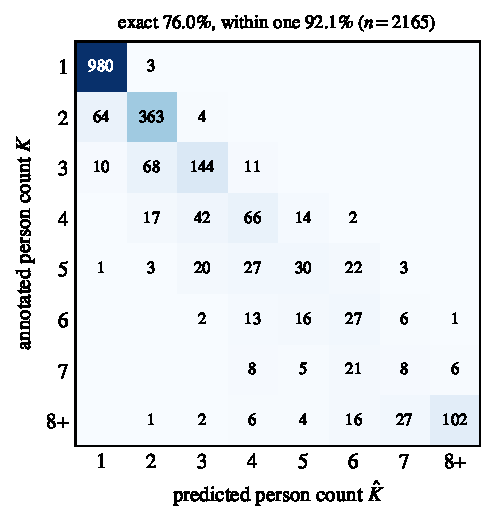
\includegraphics[width=0.64\linewidth]{figures/k_confusion.pdf}
    \caption[Predicted against annotated person count for the K head on HigherHRNet detections.]{Predicted person count $\hat{K}$ from the frozen K head against the annotated count $K$
    on the $2{,}165$ scored HigherHRNet scenes.
    Counts of eight or more are pooled into the last row and column.
    Mass below the diagonal is under-counting.
    The matrix comes from a re-run of the pipeline that reproduces the reported aggregates
    to within $0.0003$ PGA;
    two scenes receive a different count than in the logged run,
    which is why the exact-count rate reads $76.0\%$ here against $76.1\%$ in the text.}
    \label{fig:k_confusion}
\end{figure}

At first sight, a predicted cluster count outperforming the
ground-truth count appears counter-intuitive.
The distinction is that the ground-truth $K$ describes the people
annotated in the image,
whereas $k$-means operates only on the keypoints that survive detection
and matching.
Under the 10-pixel matching threshold,
HigherHRNet recovers $53{,}131$ of $66{,}998$ evaluated ground-truth
keypoints,
corresponding to $79.3\%$ recall.
The graph presented to PG-GAT is therefore an incomplete representation
of the annotated scene.

One plausible explanation for the $0.0053$ improvement is that the
annotation-level $K$ can exceed the number of people that are
meaningfully represented by the detected keypoints in some scenes.
In such cases, forcing $k$-means to use the annotation-level count may
split otherwise coherent detected groups.
The K head instead predicts from the detected embeddings
and can therefore produce a count that is better aligned with the
observed graph.
Confirming this mechanism directly would require comparing $\hat{K}$
with the number of distinct ground-truth identities represented among
the matched detections
rather than with annotation-level $K$ alone.

Regardless of the cause of the small improvement,
the autonomous result establishes the operational result required by
Section~\ref{sec_meth_integration} -
the complete pipeline can produce person-grouped keypoints without
using ground-truth information at inference.
Its PGA of $0.9644$ leaves a difference of $0.0203$ to HigherHRNet's
native AE grouping on the same evaluation protocol
and is the final autonomous result of the experimental investigation.
Figure~\ref{fig:e2e_examples} shows the three groupings on four scored scenes.

\begin{figure}[H]
    \centering
    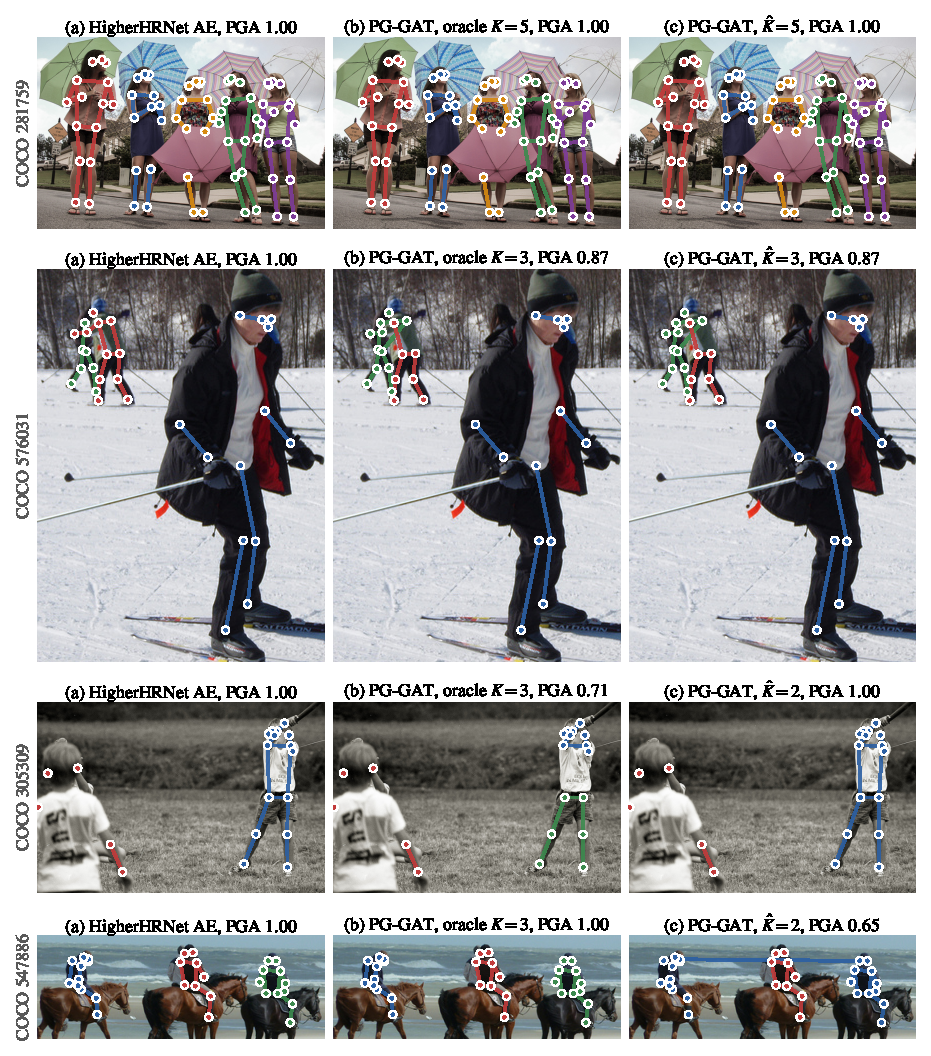
\includegraphics[width=0.97\linewidth]{figures/e2e_examples.pdf}
    \caption[Four scored COCO scenes under the three end-to-end groupings.]{Four scored COCO \texttt{val2017} scenes under the end-to-end protocol:
    (a) HigherHRNet's native AE grouping,
    (b) PG-GAT with $k$-means at the annotated $K$,
    and (c) PG-GAT with the K head's $\hat{K}$.
    Only the detections matched to ground truth are drawn,
    coloured by the person their cluster is assigned to under Hungarian matching,
    so a joint in another person's colour is a grouping error -
    the PGA in each title is the per-scene value.
    From the top: five people grouped correctly by all three;
    a grouping error at the correct count;
    a third annotated person with no matched detections,
    so the annotated $K$ splits a person while the K head's $\hat{K}=2$ does not;
    and an under-count that merges two people.}
    \label{fig:e2e_examples}
\end{figure}

\subsection{Relationship between PGA and AP@OKS}
\label{sec_res_e2e_ap}

The grouping baselines reviewed in Chapter~\ref{chap_2} are primarily
reported using AP under the OKS threshold family,
whereas the results in this chapter use PGA.
The two metrics evaluate different parts of the pose-estimation problem,
and their numerical values are therefore not directly comparable.

AP@OKS evaluates the complete pose-estimation pipeline.
A predicted person instance receives credit according to the similarity
between its assembled keypoints and a ground-truth pose under the OKS
criterion.
Detection failures,
keypoint localisation errors,
and incorrect grouping can therefore all reduce AP.
PGA instead conditions on the set of detections that have already been
matched to ground-truth keypoints
and evaluates whether those detections are assigned to the correct
person (Section~\ref{sec_meth_integration_e2e_metric}).
It consequently removes detection recall and localisation error from
the quantity being measured
and isolates the grouping decision more directly.

Grouping errors also affect the two metrics differently.
Under PGA, an incorrectly grouped keypoint contributes directly
as an incorrect assignment.
Under AP@OKS, the effect depends on how that error changes the
assembled person instances.
For example, exchanging keypoints between two people can reduce
the OKS of both predicted poses
and may therefore affect the AP contribution of both instances.
A fixed change in PGA consequently has no fixed numerical correspondence
to a change in AP@OKS.

HigherHRNet provides a useful reference between the two evaluation
views.
For the W32-512 configuration,
HigherHRNet reports an AP of $0.671$ on COCO \texttt{val2017} under its
published single-scale evaluation with flip testing~\cite{cheng2020higherhrnet},
while its native AE grouping reaches $0.9847$ PGA under the
matched-detection protocol used in this work.
These values should not be interpreted as a formal decomposition of AP,
since the metrics and evaluation procedures differ.
They nevertheless show that, once HigherHRNet keypoints have been
successfully detected and matched, its native grouping mechanism makes
relatively few person-assignment errors.
The substantially lower end-to-end AP must therefore reflect error
sources that PGA intentionally excludes,
in addition to any grouping errors that remain.

This distinction explains the use of PGA as the primary metric in the
present investigation.
PG-GAT replaces the grouping stage rather than the upstream keypoint
detector,
so PGA measures the component of the pipeline that the proposed method
is designed to change.
Reporting AP@OKS for the complete modular system would still be useful
as a system-level evaluation,
but changes in that metric would combine PG-GAT's grouping behaviour
with detection and localisation errors inherited unchanged from the
upstream detector.
PGA is therefore used to isolate the contribution of the grouping method,
while AP@OKS remains the appropriate metric for comparison of complete
pose-estimation systems.

\subsection{Detector-swap evaluation}
\label{sec_res_e2e_swap}

This section reports the detector-swap experiment of
Section~\ref{sec_meth_integration_swap}.
The same frozen \texttt{meng-headline} checkpoint and frozen K head
are applied zero-shot to detections from two additional pose detectors
belonging to different architectural families.
Neither detector contributed training examples to PG-GAT
or to the K-estimation head.

\begin{table}[H]
\centering
\footnotesize
\begin{tabular}{lccccc}
\toprule
Detector (family) & Recall & Native & PG-GAT (oracle $K$) &
PG-GAT (pred.\ $K$) & Gap \\
\midrule
HigherHRNet-W32-512 (heatmap $+$ AE)
    & 0.793 & 0.9847 & 0.9591 & 0.9644 & 0.0203 \\
YOLO11x-pose (single-stage regression)
    & 0.816 & 0.9863 & 0.9647 & 0.9653 & 0.0210 \\
RTMO-L (one-stage bottom-up)
    & 0.774 & 0.9961 & 0.9437 & 0.9741 & 0.0220 \\
\bottomrule
\end{tabular}
\caption[Detector-swap results on COCO \texttt{val2017}.]{Detector-swap results on COCO \texttt{val2017}. Native
denotes each detector's original person assignment evaluated on its
matched-detection subset. The PG-GAT columns discard these assignments,
pool the detected keypoints,
and re-group them using the same frozen \texttt{meng-headline} checkpoint,
with $K$ either taken from the ground truth or predicted by the frozen
K head. Gap is the difference between native grouping and autonomous
predicted-$K$ PG-GAT. The matched subsets contain $2{,}165$,
$2{,}196$, and $2{,}121$ scored images for HigherHRNet,
YOLO11x-pose, and RTMO-L respectively.
Consequently, comparisons between native and PG-GAT are matched within
each detector row, while absolute PGA values should be compared across
detectors with caution. The RTMO native reference uses the publicly
released multi-dataset \texttt{body7} weights.}
\label{tab:e2e_detector_swap}
\end{table}

Two findings follow from Table~\ref{tab:e2e_detector_swap}.

\textbf{1. The gap to detector-native grouping is stable across
detector families:}
The autonomous PG-GAT pipeline trails each detector's native grouping
by $0.0203$,
$0.0210$, and $0.0220$ PGA for HigherHRNet,
YOLO11x-pose, and RTMO-L respectively.
The spread between these three gaps is only $0.0017$ -
despite substantial differences in how the detectors produce and group
their keypoints.

This result provides the direct empirical test of the detector-swap
claim introduced in Section~\ref{sec_meth_integration_swap}.
PG-GAT and the K head are unchanged between all three evaluations
and operate only on the pooled keypoint coordinates,
joint types,
and associated input features.
In particular, neither component is retrained or adapted to
YOLO11x-pose or RTMO-L.
The fact that the autonomous pipeline remains within approximately
$0.02$ PGA of native grouping across all three detectors shows that
its performance is not specific to the HigherHRNet candidate
distribution on which the original end-to-end evaluation was performed.

The gap should not be interpreted as a direct numerical measurement
of the cost of modularity alone.
Each native grouping mechanism differs from PG-GAT in its representation,
training data,
objective,
and access to detector-internal features.
What the experiment establishes is that replacing these detector-specific
assignments with the same external grouping module incurs a small,
and remarkably consistent, empirical gap across the three detector
families tested.
For YOLO11x-pose and RTMO-L, the native person assignment is also
produced as part of the detector itself rather than by a detachable
grouping module.
PG-GAT therefore provides a form of interchangeability that the native
assignments do not.

\textbf{2. The behaviour of predicted $K$ is consistent with an
effective-person-count effect:}
The difference between predicted-$K$ and oracle-$K$ PG-GAT changes
substantially with the detector.
For YOLO11x-pose, which has the highest matched-keypoint recall
at $0.816$, predicted $K$ changes PGA by only $+0.0006$.
For HigherHRNet at $0.793$ recall, the difference increases to
$+0.0053$, while for RTMO-L at $0.774$ recall it reaches $+0.0304$.
In the ground-truth-keypoint evaluation, where the input contains
the annotated keypoints rather than an incomplete detector output,
predicted $K$ instead trails the true count by $0.0066$.

These four operating points form a monotonic pattern -
as the keypoint set becomes less complete,
the annotation-level person count becomes less useful as the cluster
count for the graph actually presented to PG-GAT,
while the count estimated from that graph becomes relatively more useful.
This behaviour is consistent with the explanation proposed in the
HigherHRNet experiment.
If some annotated people are only weakly represented among the surviving
detections, forcing $k$-means to use the annotation-level $K$ can
introduce unnecessary clusters and split otherwise coherent detected groups.
The K head, which predicts from the observed embeddings, can instead
return a count closer to the number of people represented strongly
enough to support grouping.

The detector swap strengthens this interpretation because the same
trend appears across three independently generated detection sets
and reverses in the ground-truth-keypoint control.
It does not, however, prove that recall alone causes the effect -
detector identity,
visibility patterns,
localisation errors,
and the distribution of missing joints also change between the three rows.
A direct test would compare both $K$ and $\hat{K}$ with the number
of distinct ground-truth identities represented by the matched
detections in each scene.
The present result is therefore evidence consistent with the
effective-person-count explanation
rather than a causal isolation of that mechanism.
\section{Model Size and Modularity}
\label{sec_res_model_size}

Parameter counts: PG-GAT 170{,}560; K-head 18{,}625; HigherHRNet-W32 full model 28{,}645{,}331; HigherHRNet AE tag head alone $\sim$561. Correction to the earlier ``168$\times$ smaller'' claim: PG-GAT is \emph{larger} than the pure AE tag head (170K vs 561). The contribution is modularity --- PG-GAT plugs into any detector's keypoint output without joint training; the AE head cannot.

\section{PG-GAT v2 --- Visual Feature Augmentation}
\label{sec_res_v2}

This section reports the result for the visual-feature-augmented PG-GAT variant of Section~\ref{sec_meth_v2}.
The hypothesis under test is that pre-trained ImageNet features sampled at each keypoint location
add identity signal that the positional input of Section~\ref{sec_meth_problem_graph} cannot provide.
The result is a documented negative:
visual features lift COCO grouping by less than one point while adding $2.2 \times 10^{6}$ MobileNet parameters to the pipeline,
and the resulting model size exceeds HigherHRNet's while still scoring below it.

\subsection{Setup}
\label{sec_res_v2_setup}

Two training schedules are reported:
the 20-epoch initial schedule at learning rate $10^{-3}$ with cosine decay to $10^{-5}$,
and the 50-epoch extended schedule that resumes from the 20-epoch checkpoint at a halved initial learning rate $5 \times 10^{-4}$ and continues for 30 additional epochs.
Both train on the cached COCO MobileNetV2 features of Section~\ref{sec_meth_v2_features}
(54{,}564 training samples, 2{,}258 validation samples)
with the contrastive loss of Equation~\eqref{eq:contrastive_loss} only.
The MobileNetV2 backbone is held frozen throughout;
the visual-feature projection block of Equation~\eqref{eq:v2_projection} is trained jointly with the GAT.
Validation runs every two epochs on the cached COCO validation features.

\subsection{Headline numbers}
\label{sec_res_v2_numbers}

\begin{table}[H]
\centering
\footnotesize
\begin{tabular}{lccl}
\toprule
Configuration & COCO val PGA (kNN, GT kp) & Param count & W\&B run \\
\midrule
PG-GAT v1 (\texttt{meng-headline}, no visual features) & 0.9715 & 170{,}560        & \texttt{b5noyg7t} \\
PG-GAT v2, 20-epoch                                    & 0.9731 & 197{,}280 + 2.2M MobileNet  & \texttt{vg43ee4u} \\
PG-GAT v2, 50-epoch extended                           & 0.9749 & 197{,}280 + 2.2M MobileNet  & \texttt{o8978au7} \\
\midrule
HigherHRNet AE (reference upper bound)                 & --- & 28{,}645{,}331 & --- \\
\bottomrule
\end{tabular}
\caption{PG-GAT v2 against the no-visual-features PG-GAT headline and the HigherHRNet AE reference.
The v2 lift over the headline is $+0.0034$ COCO val PGA (50-epoch extended);
the MobileNetV2 backbone that produces the visual features contributes a further $2.2 \times 10^{6}$ parameters
to the total pipeline size.}
\label{tab:v2_headline}
\end{table}

\subsection{Interpretation}
\label{sec_res_v2_discussion}

Three observations.

\paragraph{1. The visual signal is real but small.}
The 20-epoch v2 number ($0.9731$) is $+0.0016$ above the no-visual-features headline ($0.9715$),
and the 50-epoch extended run lifts to $0.9749$ for an additional $+0.0018$ over the 20-epoch result and a total lift of $+0.0034$ over the headline.
Both differences are above the per-image standard deviation of the metric,
which means the visual signal is contributing a measurable lift in absolute terms.
The 50-epoch extended run rules out the possibility that the v2 architecture is undertrained at 20 epochs;
the additional 30 epochs add $+0.0018$ COCO val PGA,
which is statistically detectable but practically negligible.

\paragraph{2. The lift is bought at substantial parameter cost.}
The PG-GAT v2 network itself adds approximately $27{,}000$ parameters over the baseline PG-GAT
(the projection block of Equation~\eqref{eq:v2_projection} plus the adjusted first GAT layer).
The MobileNet backbone that supplies the visual features adds a further $2.2 \times 10^{6}$ parameters,
all of which must be present at inference time to compute the visual features for new images.
The total deployable pipeline therefore consists of approximately $30.8 \times 10^{6}$ parameters
(HigherHRNet detector $28.6 \times 10^{6}$ + MobileNet backbone $2.2 \times 10^{6}$ + PG-GAT v2 network $0.2 \times 10^{6}$),
which exceeds HigherHRNet's all-in size of $28.6 \times 10^{6}$ while producing a COCO PGA below HigherHRNet's $0.9847$.
The size accounting is the subject of Section~\ref{sec_res_model_size};
the empirical bottom-line is that the trade is unfavourable.

\paragraph{3. The result is reported as a negative finding.}
The hypothesis under test was that visual features would push the modular PG-GAT pipeline past the HigherHRNet AE reference of $0.9847$.
The result is $0.9749$ at the 50-epoch extended run,
which is $0.0098$ below the AE reference and only $0.0034$ above the no-visual-features PG-GAT.
The visual signal exists but is insufficient to close the gap to AE,
and the price in parameter count exceeds the price the HigherHRNet AE alternative pays in total pipeline size.
On this evidence, visual-feature augmentation is not pursued as a follow-on research direction;
the result is reported here in full so that future work that revisits visual augmentation
(for example with a larger backbone, or end-to-end joint training of backbone and grouping network)
has a clear baseline to beat.


%% End of File.
